\subsection{Concepts de base: }
La base de données HBase est régie par les concepts suivants :

\begin{itemize}[label=\textbullet]

\item \textbf{Map :} Le stockage se fait dans une map. Cette dernière est basée sur le principe de clé/valeur. Chaque valeur (tableau de bytes) est identifiée par une clé (tableau de bytes). L'accès a une valeur par sa clé est très rapide.

\item \textbf{Map trié :} La map est triée par ordre lexicographique. Cette fonctionnalité de tri est très importante car elle permet de récupérer les valeurs par intervalle de clés.
\item Multidimensionnel : La clé dans la map est une structurée composée de row-key, column family, column, et d'un timestamp.

\item \textbf{Multidimensionnel :} La clé dans la map est une structure composée de row-key,
column family, column, et d'un timestamp.

\begin{figure}[h]
	\centering
    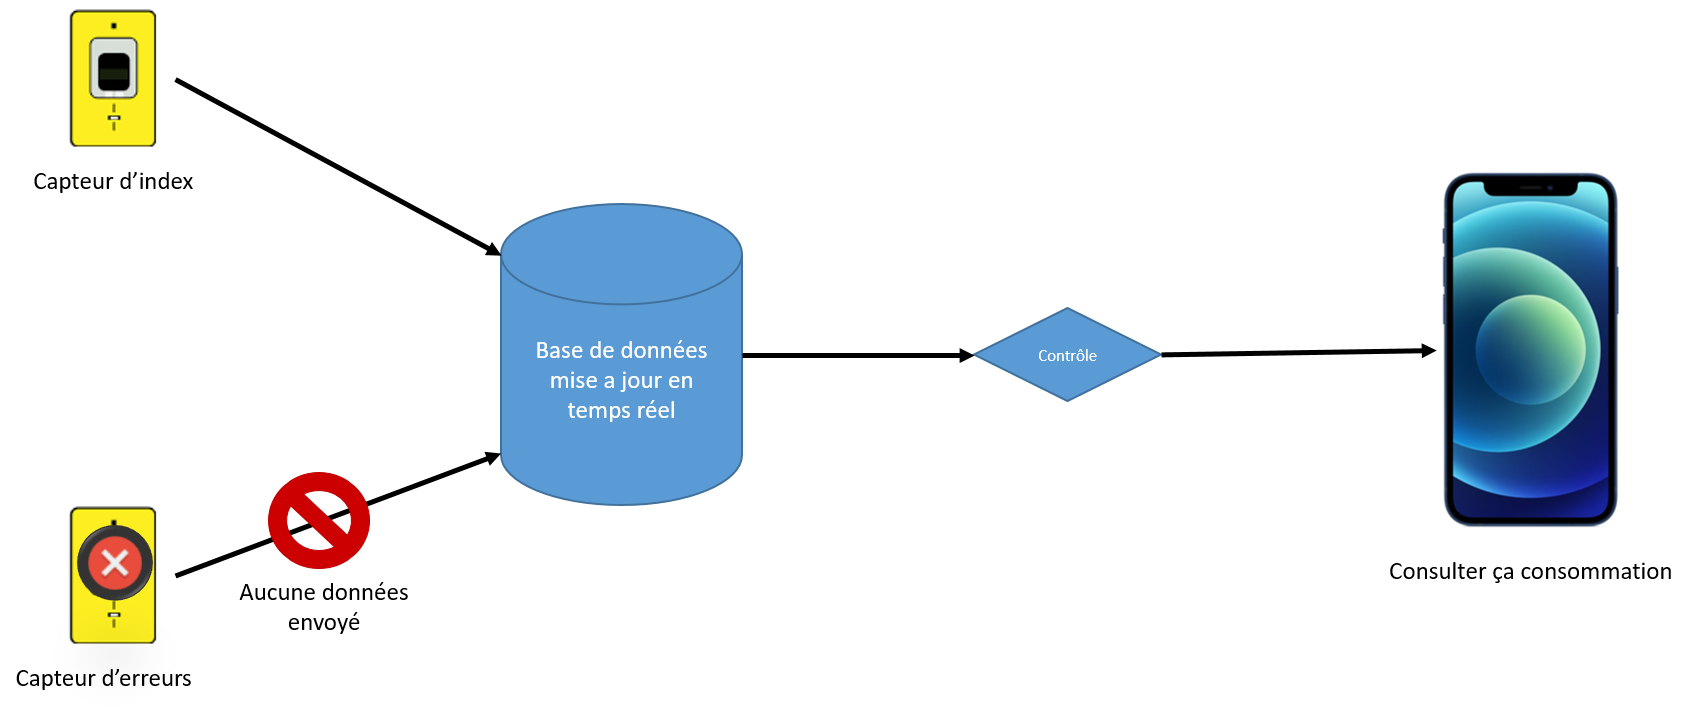
\includegraphics[scale=0.4]{img/part2/2.1}
    \caption{Structure d'une clé dans la map}
\end{figure}

\item \textbf{Null (Sparse) :} Contrairement aux bases de données relationnelles, une colonne qui n'a pas de valeur n'est pas matérialisée (aucun stockage n'est nécessaire en cas d'une valeur null pour une colonne).

\item \textbf{Persistance :} Les données stockées dans la map sont sauvegardées durablement sur disque.

\item \textbf{Consistance :} Toutes les modifications sont atomiques et les lectures se font toujours sur la dernière valeur validée (commit).

\item \textbf{Système distribué :} Le système de base de données est construit sur un systèmes de fichiers distribués afin que le stockage de fichiers sous-jacent soit reparti sur un ensemble de machines d'un cluster. Les données sont répliquées sur un certain nombre de nœuds permettant ainsi une tolérance aux pannes.
\end{itemize}